\section{Introduction}
\begin{quotation}
\textit{Imagine an earthquake has hit a populous area and many major roads are
impassable. Buildings are serverly damaged or collapsed, and fire has broken out
in many places. At the crisis management center, response professionals are
working together to coordinate the earthquake relief effort. You are the
incident commander charged with coordinating the search
and rescue teams working in the field. There is a large tabletop display in
front of you, showing the map of the site. Information coming from the field is
updated on the display in real-time.}

\textit{A report about a big explosion at a chemical plant comes in and you move
the map around, zoom in and rotate it to get a good view of the plant. On the
map, you see there is a group of unmanned vehicles nearby. After selecting them
on the map with your hand, you speak to the interface ``Go nearer to the
explosion site to gather more information,'' while tracing the route the
vehicles should take to avoid obstacles. Then you instruct rescue team No. 3 to evacuate the residents
in the sorrounding buildings by going under a bridge because the surface of the
bridge is blocked. You gesture with one hand as the bridge and the other
hand moving under it to emphasize this.}
\end{quotation}

The scenario above shows an application of a multi-modal interface to a
real-world problem. Gestures play an important part in this scenario,
providing key information about location, method and timing of movements,
and about spatial relationship among the objects being described.

Recent trends in user interfaces have brought on a new wave of interaction
techniques that depart from the traditional mouse and keyboard that have been 
used for decades. These include multi-touch interfaces such as the 
iPhone\textsuperscript{\textregistered}, iPad and the Microsoft 
Surface\textsuperscript{\textregistered} as well as camera-based systems such as
the Microsoft Kinect and the Nintendo\textsuperscript{\textregistered} Wii. Most
of these devices gained instant popularity among consumers, and the common trait
among them is that they make interacting with computation more natural and 
effortless. All these devices allow users to use their hands and/or body 
gestures to directly manipulate the virtual objects. It feels more natural this 
way because this is how we interact with our environment in everyday life.
 
Our goal is to take this aspiration to the next level by developing an
intelligent multimodal interface for natural interaction. By \textit{natural
interaction}, we mean the kind of cognitively transparent, effortless multimodal
communication that can happen between people; we want to make this possible in
human-computer interaction such that the computer interface understands what the
user is saying and doing, and the user can simply behave. We believe that
natural interaction can provide better learnability, flexibility, memorability,
convenience and efficiency, but further user studies are needed to investigate
this belief.

Gesture plays an important part in multimodal interaction, especially for
conveying spatial information. The focus of this thesis is developing a
hierarchical approach for continous gesture analysis that can be easily
applied in different domains and applications. Specifically, we focus on
gestures made with hands.

\section{Background}
In thier review of visual interpretation of hand gestures for HCI, Pavlovic
\cite{Pavlovic97} et al. states that hand gestures in natural environments are
used for both manipulative actions and communication. However, the communicative
role of gestures is subtle, since hand gestures tend to be a supportive element 
of speech (with the exception of deictic gestures, which play a major role in 
human communication).

\section{Related Work}
There are many active research on using hand as an input modality for
human-computer interaction. To do this, the computer needs to be able to
interpret the dynamic and/or static configurations of the human hand, arm, and
even other parts fo the human body. (Mention Kettebekov's paper and the
framework. Gesture definition.)

\subsection{Sensors}
The first step in the pipeline is having sensors that captures the hand movement
and configurations, converting analog signals to digital signals. First attemps
to solve this problem resulted in mechanical devices that directly measure hand
joint angles and spatial position. This group is best represented by the
glove-based approaches using divecs such us CyberGloves \cite{fels09} and
Powergloves \cite{kadous02}. However, wearing gloves makes gesturing more
combersome and many efforts have been to make the gloves more light-weight by
using bluetooth wireless data transmission (e.g. CyberGove II). To further
reduce the bulkyness of the gloves, people use colored markers on the fingers
\cite{mistry09} or colored gloves with not electronics \cite{Wang09} and use RGB
cameras and computer vision techniques to interpret gestures. However, by
requiring the user wearing something additional still hinders the acceptance of
such device as a ``everyday'' natural interaction interface. 

The most nonobtrusive way to capture the hand is bare-hand tracking. People have
used different types of camera to achive this task. \cite{Shin04} used stereo RGB
cameras to extract the hand from background based on the skin color. One
limitation of use RGB cameras is they are very sensitive to lighting conditions.
This prompted researchers to look into other types of cameras. Oka et al. 
\cite{Oka02} uses thermal imaging for hand segmentation under compplex
background and changing light, relying on the condition that a hand's
temperature is almost always distince from the background. Their approach does
not detect finger contact with the surface. Larson et al. \cite{larson11}
improves on this method to detect the finger contact by using
the heat transferred from a user's hand to the surface for touch-based gestures.
However, inorder to detect the head trace, the user has to drag the fingers a
bit instead of just touching. This may be a small departure from what the user
would expect as ``natural'' based on the experience in the physical world.

Thermal imaging measures radiation emitted by objects in the F-IR spectrum.
There are other well-known ``IR-imaging'' techniques used in the HCI community
which use device that operate in the \textit{near}0-infrared (N-IR) spectrum.
N-IR is employed in some fairly recent interactive tabletop surfaces and depth
cameras. A number of project in the HCI community have used IR for tabletop
interaction by detecting multi-touch gestures using an under mounted
camera and illumination source. An exmaple of this is Microsoft's 
Surface\textsuperscript{\textregistered}. Recently portable multi-touch devices
such as phones and tablets have become more and more ubiquitous. These devices
are based on capacitve touch sensitive screens. Touch-based devices are becoming
more and more mature, however the kind of gestures one can use are still
limited. The gestures are usually limited in 2D space with one or multiple
fingers. 

Going beyond the limitation of touch-only gesture, researchers at Microsoft
augmented the Surface technology with a switchable diffuser, additional
strips of IR LEDS with a different wave length for diffuse illumination, and an
additional IR sensitive camera which images IR reflected from the diffuse
illumination of the environment \cite{hilliges09}. In this way, they can capture
the hand above the surface as well. The height of the hand is estimated based on
the pixel intensity.

Since the introduction of Kinect, a motion sensing inut device by Microsoft for
the Xbox 360 video game console, researchers in the HCI community, as well as
many independent hackers, have been using Kinect's depth sensor for capturing
both body and hand gestures \cite{openni}. Since then, there are also many
similar devices coming into the market which have been used for capturing
gestures. For instance, Harrison et al. \cite{harrison11} uses  a short-range
PrimeSense \cite{primesense} depth camera for their wearable multitouch
interaction. In comparison to the aforementioned augmented Surface setup,
Kinect, and the likes, provides a cheap alternative for depth sensing. In this
thesis, we will explore the potential of using the Kinect sensor for detecting 
both the touch-based gesture and above-surface 3D gestures. Potentially, we can 
use the depth information for determing surface touch, and hence, eliminate the 
need for the complicated electronics of a touch sensitive screen. This also 
enables the gestural interaction on a large tabletop display, much bigger than 
that of Microsoft's Surface.

\subsection{Hand tracking}
After getting input from the sensor(s), the next step in the pipeline is
tracking the hand(s). This is essentially the frame-by-frame estimation of the
parameters of the hand model based on the sensor input. The complexity of the
hand model is application dependent. For a given application, a very coarse and
simple model may be sufficient. The simplest model is treating the hand as a
blob and only the 2D/3D location of the blob is tracked. For example, Sharma et
al. \cite{sharma00} used 2D positional and time differential parameters to track
the hands as blobs which was sufficient for them to distinguish whether the
hands were doing a point, contour or circle gesture. PrimeSense NITE requires the user to do a ``focus'' gesture (``click'' or
``wave'') to gain control and start hand-tracking \cite{primesense-manual}. The
gestures it supports are ``click'', ``wave'', ``swipe left'', ``swipe right'',
``raise hand candidate'' and ``hand candidate moved''.

However, to make a more generalizable system for natural-like interaction, a
more sophisticated model is required. One step forward is adding fingertips
location in the hand model as exmplified in \cite{Oka02} \cite{harrison11}
\cite{larson11}. Tracking fingertips is usually sufficient for manipulating
objects on the 2D surface. However, for a more rich set of gestures, the one
that also involves communicative gestures, we may need a more sophisticated
model. Wang et al. \cite{Wang09} uses a 26 degree of freedom (DOF) 3-D skeletal
model in their real-time hand-tracking system. 

Another approach is using appearance-based model. This means that the model
parameters are not directly derived from the 3D spatial description of the hand.
The gestures are modeled by relating the appearance of any gesture to the 
appearance of the set of predefined, template gestures \cite{Pavlovic97}. In
their markless hand tracking system, Wang et al. \cite{wang11} uses efficient
queries of a database of gesture and desktop-specific hand silhouette samples
for pinch/click gesture detection.

In our system, we propose a combination of both approaches. A 3-D skeletal hand
model is useful for manipulative gestures because we want to know exactly where
the fingertips are and the grabbing and releasing poses of the hand. For
communicative gestures, we just need to know the meaning of the gesture instead
of the exact spatial parameters. Hence a example template model would be more
suitable which may require less computation.

\subsection{Gesture recognition}
Most of the gestural input applications have been focusing on tracking only
\cite{harrison11} \cite{larson11}. For hand gesture recognition, much of the
work is on sythetic gestures, most notably sign language recognition
\cite{Bauer00} \cite{kadous02}. Wang et al. \cite{Wang09} made a simple
demonstration fo sign language finger spelling with their color glove hand-tracking system. 
For dynamic gesture recognition, hidden markov model (HMM) is a commonly used
technique because it is suitable for time series data \cite{sharma00}. 

Wang et al. \cite{wang06} argued that a significant limitation of the
HMM is the requirement of conditional independence of observations. In
addition, HMM, as a generative model, optimizes the likehood of
generating all the examples of a given gesture class, which is not
necessarily optimal for discriminating the gesture class against other
gestures. They introduced the use of hidden conditional random fields (HCRF) for
gesture recognition, and and showed improved accuracy for the set of head and
arm gestures they use compared with using HMMs. 

On the topic of discriminative vs. generative classifiers, Ng and Jordan
\cite{ng02} shows that while discriminative learning has lower asymptotic error,
a generative classifier may also approachy its higher asymptotic error much
faster. Their claim is based on experiments with the naive Bayes classifier and
logistic regression Generative-Discriminative pair. This means the performance
of the two kinds of classifiers may be dependent on the number of training
examples. In this thesis, we will compare both the HMM and HCRF approach and
analyze their performance based on the number of training examples.

There are few work that actually distinguishes manipulative gestures and
communcative gestures. Oka et al. \cite{Oka02} developed a system that allows
both direct manipulation and symbolic gestures. Based on the tracking result,
the system first differentiates the gesture as either manipulative or symbolic 
according to the extension of the thumb. They regard gestures with an extended 
thumb as direct manipulation and those with a bent thumb as symbolic gestures. 
For direnct manipulation, the system selects operating modes such as rotate, 
move or resize based on the fingertips configuration; for symbolic gestures, it 
uses HMM for classification. The way they distinguish manipulative and 
communicative gestures seems to be arbitrary and ``unnatural''. They did that 
probably for the ease of it because they are only trakcing fingertips.

We propose an interface that can seamlessly switching between between
manipulative and communcative gestures based on the learned parameters. We
believe the distinction among different classes of getures is useful for the
input system because the best parameter space may be different for different
classes. This motivate our hierachical approach to continuous gesture
recognition.

\subsection{Multimodal systems}
Bolt's pioneering work in the ``Put That There'' system \cite{Bolt80} 
demonstrated the potential for voice and gestural interaction.  In that system, 
the hand position and orientation was tracked by the Polhemus tracker, i.e., the
hand was essentially transformed to a point on the screening. The actual hand 
posture did not matter, even if it was not in a pointing shape. The speech also 
followed a rigid and limited command-like grammar. Even though this is an early 
work, it provides some insight about the advantages of multimodal interaction. 
As Bolt summarized in the paper, using pointing gesture allows the use of 
pronouns in the speech, with the corresponding gain in naturalness and economy 
of expression \cite{Bolt80}.

Since then, several multi-modal interaction prototypes were 
developed that moved beyond Bolt's ``Put That There'' system. Cohen et al. 
\cite{Cohen97} developed the QuickSet prototype which is a collaborative, 
multimodal system running on a hand-held PC using pen and voice as input. They 
used a novel multimodal integration strategy that allows speech and pen gesture 
to compensate for each other, yielding a more robust system. Rauschert et al. 
\cite{Rauschert02} developed a system called Dialogue-Assisted Visual 
Environment for Geoinformation (DAVE\_G) that uses free hand gestures and speech
as input. They recognized that gestures are more useful for expressing spatial 
relations and locations. Gestures in DAVE\_G included pointing, indicating an 
area and outlining contours. Speech and gesture are fused for commands that need
spatial information provided by the gesture. 

In this thesis, we will also explore the fusion of speech gestures. In addition
to use the deicitc gestures to provide spatial information as a complement to
speech as in \cite{Rauschert02}, we will also explore the the use of speech as a
complement to manipulative gestures based on the finding from a user study done
by Yin et al.\cite{yin10}. They observed that manipulative gestures are at times
accompanied by adjectives and adverbs that refine the actions.

\section{Proposed Work and Procedure}
Our long term goal is to build an intelligent multimodal interface for natural
interaction that can serve as a testbed for enabling the formulation of a more
principled system design framework for multimodal HCI. One focus of this thesis
is on the gestural input modality. The user should be able to use gesture as an
input effortlessly for both direct manipulation and communication to the system.

\subsection{Gestural Taxonomy}

\subsection{Project Setup}
The custom tabletop structure includes four $1280\times1024$ pixel projectors 
(Dell 5100MP) that provide a $2560\times2048$ pixel resolution. 

\begin{figure}
	\centering
	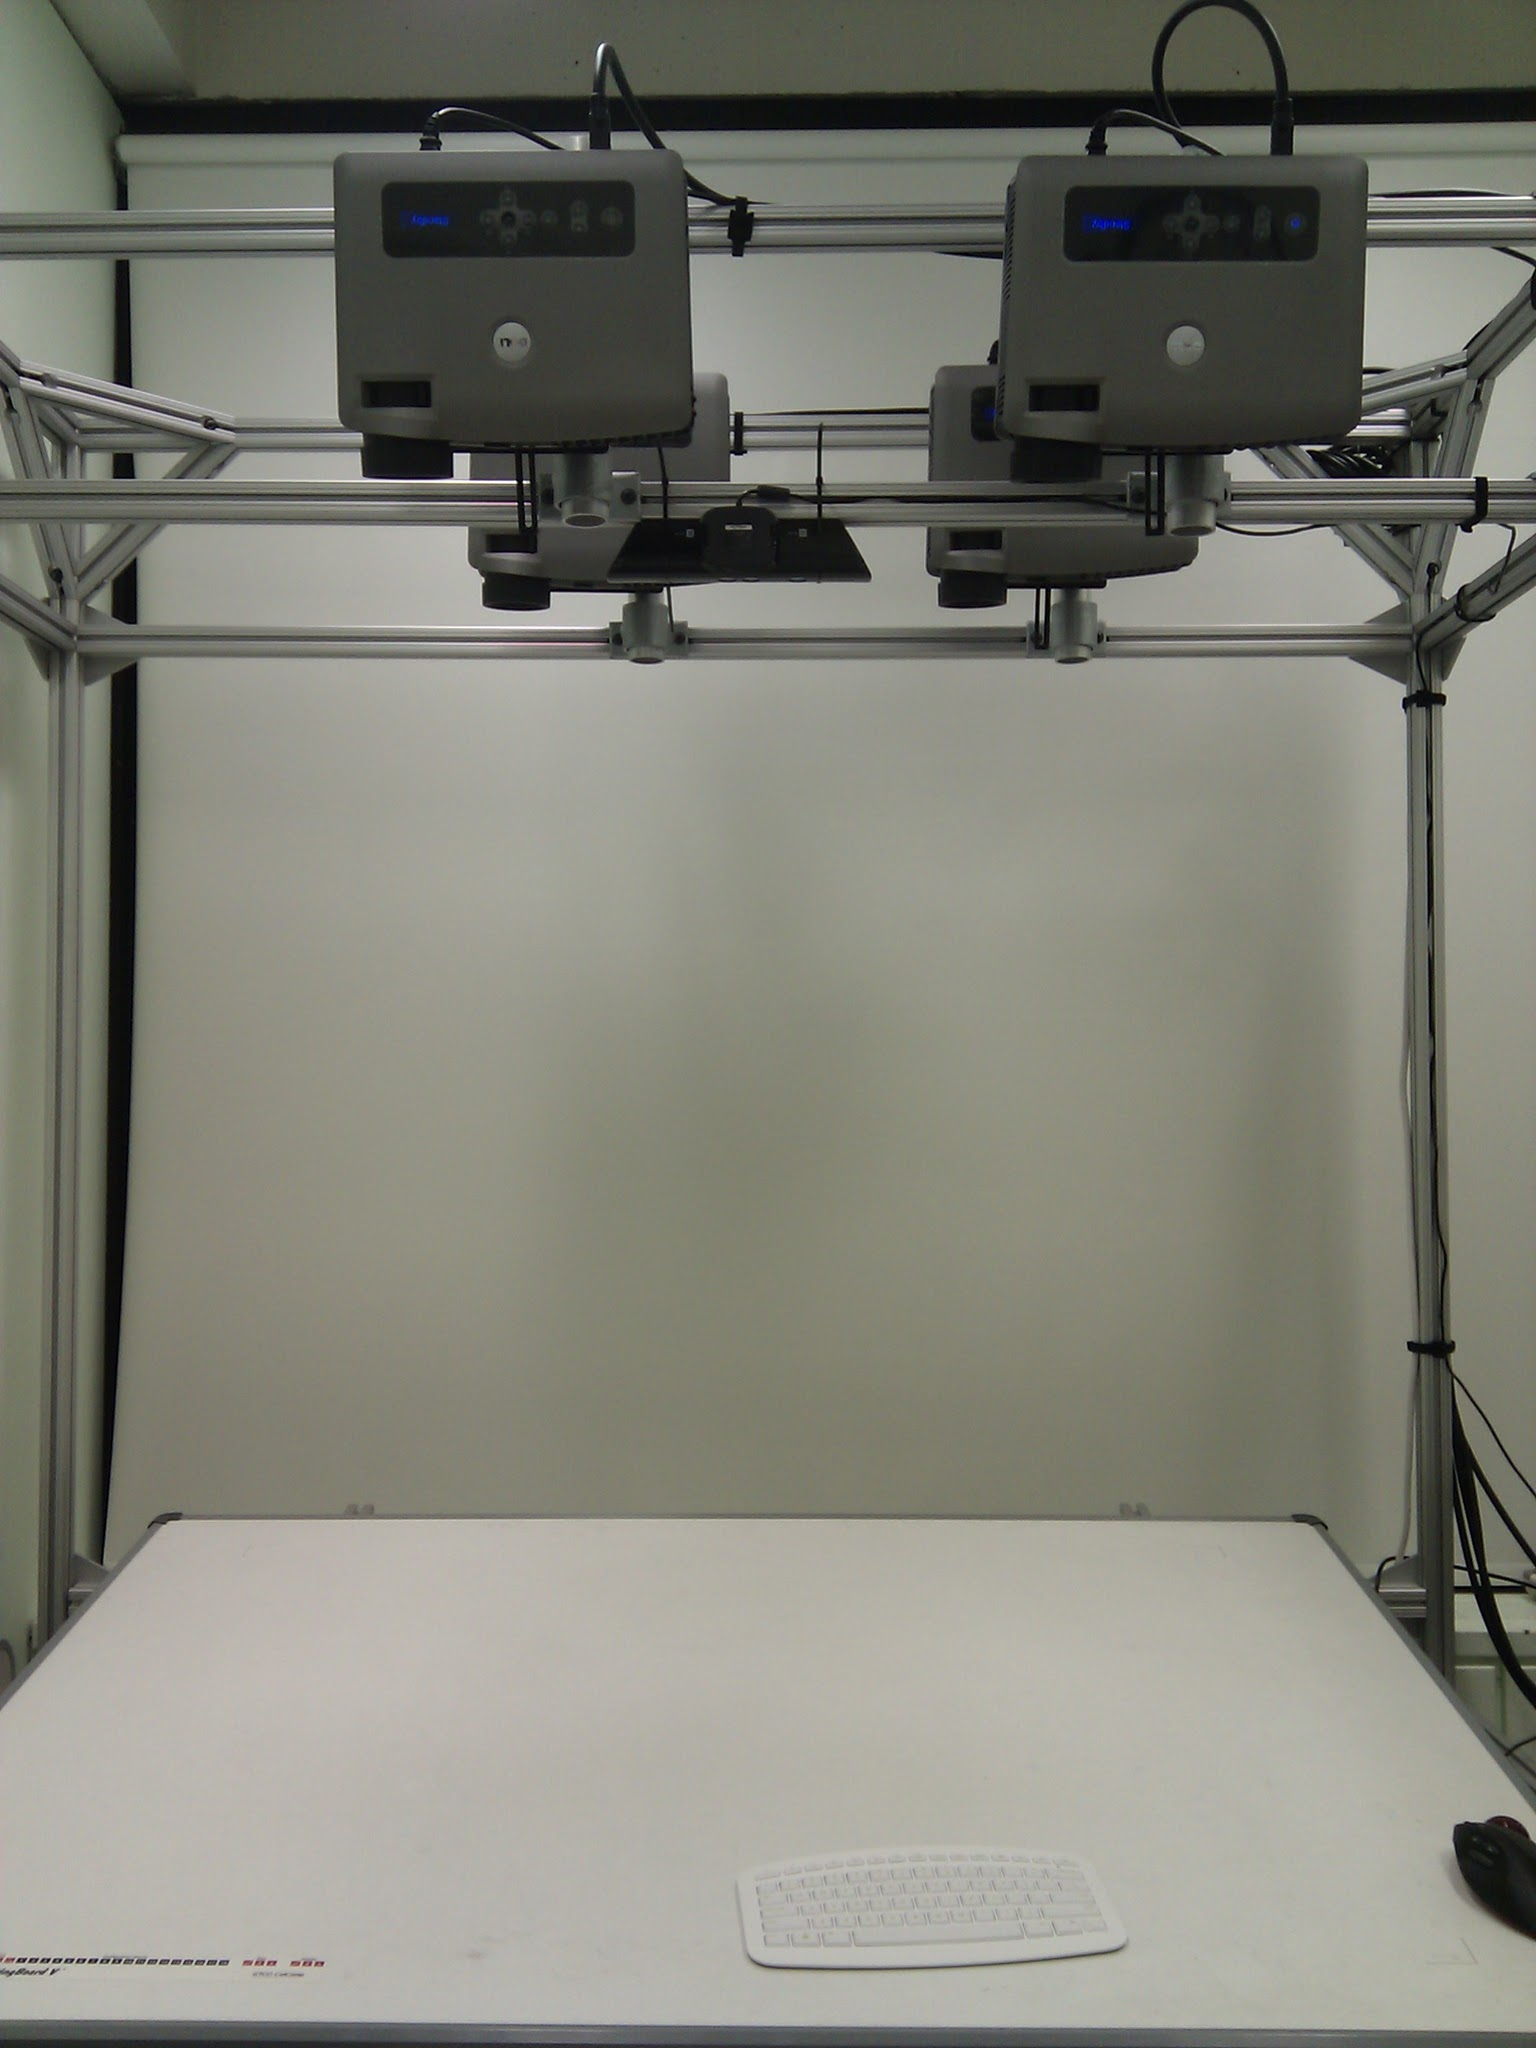
\includegraphics[width=0.7\textwidth]{figures/setup1.png} 
	\caption{System setup.} \label{fig:setup}
\end{figure}

The display is projected onto a flat white surface digitizer (GTCO Calcomp DrawingBoard V), which uses a stylus as an input device. The digitizer is tilted 10 degrees down in front, and is placed at 41in (104cm) above the floor, following FAA's design standard to accommodate the $5^{th}$ through $95^{th}$ percentiles of population. Projected displays were mechanically aligned to produce a single seamless large display area. One Fire-i\texttrademark Digital Camera from Unibrain is placed above the center of the tabletop at the same level of the projectors. We use the Google Earth web browser plug-in as our basis for 3D maps. Figure \ref{fig:setup} shows the setup.

The Dell 5100MP projector uses a spinning color wheel to modulate the image. This produces a visible artifact on the screen, referred to as the ``rainbow effect'', with colors separating out in distinct red, green, and blue. At any given instant in time, the image on the screen is either red, or green, or blue, and the technology relies upon people's eyes not being able to detect the rapid changes from one to the other. However, when seen through a camera, the effect is very obvious, and this can greatly affect the color classification for the hand tracking. To reduce this effect, the exposure rate of the camera needs to be adjusted to be a multiple of the rotation period of the color wheel. The projector uses 2x color wheel speed, which is about 120 rotation/second. Hence, the period is about 8.3ms. After adjusting the exposure rate of the camera to approximately 8.3ms, the effect is greatly mitigated, but still present. 

\subsection{Hand Tracking}
An important part of multimodal interface is acquiring valid multimodal data. The most common acquisition methods for hand gestures are magnetic trackers, cyber-gloves and vision-based approaches. Acquisition using magnetic trackers and cybergloves is efficient and accurate, but suffers from the need to wear restrictive devices. Most existing vision-based hand tracking systems track only hand movement and finger tips, rather than 3D hand posture \cite{Demirdjian03}\cite{Oka02}\cite{Rauschert02}. This limitation often requires that artificial gestures be defined for easy tracking and recognition.  

We use a different web camera from the one used by Wang. This is also a verification that the hand-tracking system is compatible and works well with different ordinary webcams. Using the FireAPI\texttrademark 1394a/1394b development toolkit, we developed a wrapper for the Fire-i camera driver to interface with the hand-tracking system. The camera is set to capture $640 \times 480$ video at 15Hz.  

Wang's hand-tracking software was developed originally for use in an office environment with standard illumination. Several interesting steps are required to use it in our context, with its complex and dynamic background (the maps) and the non-uniform illumination of the glove from the maps. 

\subsection{Background Subtraction}
To clean up the background subtracted depth image, we use morphological opening
to clear out small pixel noises. 

\subsection{Kalman Filter}
Kalman Filter is used to further improve the tracking accurcy.
Let $x_k$ be an $n$-dimentional vector of state components and $P_k$ be the
$n$-by-$n$ error covariance. The measurements $z_k$ is a $m$-dimensional
vector given by:
\begin{align*}
z_k = H_kx_k + v_k,
\end{align*}
where $H_k$ is an $m$-by-$n$ matrix and $v_k$ is the measurement error.

The \textit{Kalman gain}, $K_k$, is an $n$-by-$m$ matrix expressed as:
\begin{align*}
K_k = P_k^-H_k^T(H_kP_k^-H_k^T + R_k)^{-1}
\end{align*}

Assuming no external control, the a priori estimate $x_k^-$ of the state is
given by:
\begin{align*}
x_k^- = Fx_{k - 1} + w_k,
\end{align*}
where $F$ is the $n$-by-$n$ \textit{transfer matrix} characterizing the
dynamics of the system, and $w_k$ is the \textit{process noise} associated with
random events or forces that directly affect the actual state of the system. We assume that the components of $w_k$
have Gaussian distribution $N(0, Q_k)$ for some $n$-by-$n$ covariance matrix
$Q_k$.

Using $P_k^-$ to denote the error covariance, the a priori estimate for this
covariance at time $k$ is obtained from the value at time $k - 1$ by:
\begin{align*}
P_k^- = FP_{k - 1}F^T + Q_{k - 1}
\end{align*}

The updated value for $x_k$ when a new measurement is available is:
\begin{align*}
x_k = x_k^- + K_k(z_k^- - H_kx_k^-)
\end{align*}
The update value for $P_k$ is:
\begin{align*}
P_k = (I - K_kH_k)P_k^-
\end{align*}
   
\subsection{Gesture Recognition}
Bootstrap the system with gesture models learned from users.

How to differentiate manipulative gestures and communicative gesture.

We adopt the taxonomy of hand movements proposed by Pavlovi\'{c} et al. \cite{Pavlovic97} which distinguishes gestures from unintentional hand movements (like beats). They then further divided the gestures into manipulative and communicative classes. 

Many previous systems distinguish gestures from unintentional hand movements by restricting the hand motion or defining some arbitrary gesture to indicate the start of gesture \cite{Shin04}. With the ability to track 3D hand postures in real-time, we can train the gesture recognizer with a set of natural gestures without being worried about whether those gestures are easily recognized by the system. Any hand motion that is not classified will not have a effect on the state of the system.

Manipulative gestures are the ones used to act on objects, while communicative ones have an inherent communicational purpose\cite{Pavlovic97}. In a natural environment, communicative gestures are usually accompanied by speech. Hence, for manipulative gestures, our classification will be entirely based on the hand states, while for communicative gestures, both hand and speech recognitions will be combined for recognition. 

The output from the hand tracker is a sequence of data describing the translation (in x, y, z coordinates) and orientation (in a quaternion) of the hand and each finger joint. There are three joints per finger in the model. The joint at the base of each finger has 2 DOFs while the other two joints of each finger have 1 DOF each. From the tracker output, we derive the feature vector at each time frame. For each finger, we are interested in the bending angles of the joints. Hence, we convert the joint orientation in quaternion to Euler angles. The translation of the joint is irrelevant because it is relative to the hand and stays the same. The feature vector includes the speed of hand movement in the x-y plane (obtained from the global translation of the hand), z position of the hand, roll, pitch and yaw of the hand, and four angles for each finger (one angle for each of the first two joints and two angles for the base joint). The result is a 25-dimensional feature vector.

\begin{figure}[htp]
\begin{center}
\includegraphics[width=.7\textwidth]{figures/Bakis.jpg}
\caption{{The state transition diagram of a 4-state Bakis model with corresponding transition probabilities}}\label{fig:bakis}
\end{center}
\end{figure}

The position and the orientation of the hand through time can be assumed to follow the first order Markov process \cite{Starner95}. Hence, we use Hidden Markov Models (HMMs) to classify gestures. There exist many kinds of HMMs \cite{Rabiner86}. One that can model time-series signals whose characteristics change successively over time is called the Bakis model \cite{Bauer00} or the Left-Right model \cite{Rabiner90}, often used in speech recognition systems \cite{Bauer00}. The Bakis model allows transitions to the same state, the next state, and the one after the next state.  Figure \ref{fig:bakis} shows an example of the Bakis model with 4 states. The Bakis model topology is particularly useful for our task because it allows different gesture speeds to be compensated \cite{Bauer00}.
	
In our experiments, we used a 6-state Bakis model, and obtained training data for 11 gestures (including panning left, right and up; roll, pitch and yaw in clockwise and anticlockwise directions, and zoom in and out). There is one HMM trained for each gesture. The probability of an observed sequence is evaluated for all competing models, and the classification is based on the model that gives the highest log-likelihood. To date, we have achieved 95\% accuracy for isolated gesture recognition. 

The next important step is continuous online gesture recognition. One issue is segmenting the continuous hand movement to get gesture intervals. The HMMs are trained for isolated gestures. When these gestures are connected together, in between, there may be unintentional hand movements, the hand may be at rest, or out of the scene. We need to add these considerations into our model.

Another issue is achieving minimum time delay of gesture recognition for a real-time interactive system. Such performance is difficult to achieve because that the starting and ending points of the gesture are not known. We will use a dynamic threshold to prune the competing gesture models based on their relative log-likelihood values. In this way, we can narrow down on a particular gesture even before the gesture ends. We will experiment with different ways of computing the dynamic threshold through data analysis of training data and cross-validation.
 
\subsection{Communicative Gesture and Speech Recognition} 
For this study, we will focus more on gesture recognition and interaction. However, as communicative gestures often co-occur with speech, we may add some basic speech recognition capability to the system in order to combine speech and deictic gestures for some USAR interaction scenarios.

\subsection{Interface with Google Earth}
Using the Google Earth Plug-in and its JavaScript API,  we embedded Google Earth, a 3D digital globe, into a web page. We use the Java web browser object in the JDesktop Integration Components (JDIC) library to load the webpage. In this way, we can augment the browser and make it respond to the gesture events from the gesture recognizer and provide the corresponding actions on the map. 

\subsection{User Study}\label{sec:userStudy}
In order to develop an interface for natural interaction in USAR Command and Control, we need to first understand what kinds of spontaneous speech, drawings, and gestures people make in such scenarios. We will try to answer this question by conducting a user study under an incident command system (ICS) environment with our tabletop display system. Experimental subjects will play the role of command center personnel charged with receiving event reports coming in from the field, making appropriate updates to a map display, then communicating commands to personnel in the field. As the user study is for bootstrapping an experimental testbed, we want minimum overhead in terms of system development. Hence, no attempt will be made in this exercise to process the drawings, speech or gestures. Instead, we will videotape the subjects and record the annotations they draw, then analyze the results to find commonalities. 

\section{Schedule}
\begin{enumerate}
	\item Experiment with polarizing filters \hfill Done by Jan 31, 2010
	
	Test whether using polarizing filters can provide better result than computing the background, or maybe we can use both methods.
	
	\item Continuous online gesture recognition \hfill Done by Feb 14, 2010
	
	Improve algorithms on continuous online gesture recognition. Conduct quantitative evaluation of the recognition results. 
	
	\item Connect user interface with gesture recognition	\hfill Done by Feb 28, 2010
	
	Interface with Google Earth. Improve system response time with gesture interaction. May need to switch to more rudimentary map interface if speed is an issue for Google Earth. May add basic speech recognition.
	 
	\item User study \hfill Done by Mar 21, 2010
	
	Conduct user study described in Section \ref{sec:userStudy}.
	
	\item Write first draft of thesis report \hfill Done by Apr 15, 2010
	\item Complete thesis report	\hfill Done by Apr 30, 2010
	\end{enumerate}
	
\section{Principal Equipment and Facilities}
Here is a list of equipment and facilities needed for the study:

\begin{enumerate}
	\item A white surface digitizer (GTCO Calcomp DrawingBoard V)
	\item Four $1280\times1024$ pixel projectors (Dell 5100MP)
	\item One web camera
	\item Polarizing filters
\end{enumerate}

All the above equipment are avalaible.

